%%%%%%%%%%%%%%%%%%%%%%%%%%%%%%%%%%%%%%%%%%%%%%%%%%%%%%%%%%%%%%%%%%%%%%%%
%                                                                      %
%     File: Thesis_Results.tex                                         %
%     Tex Master: Thesis.tex                                           %
%                                                                      %
%     Author: Andre C. Marta                                           %
%     Last modified :  2 Jul 2015                                      %
%                                                                      %
%%%%%%%%%%%%%%%%%%%%%%%%%%%%%%%%%%%%%%%%%%%%%%%%%%%%%%%%%%%%%%%%%%%%%%%%

\chapter{Adding a new product when already producing one (Firm is already active before investing)}
\label{chapter:2}



%%%%%%%%%%%%%%%%%%%%%%%%%%%%%%%%%%%%%%%%%%%%%%%%%%%%%%%%%%%%%%%%%%%%%%%%
\section{Introduction}
\label{section:2_intro}

We consider now the case where, even before we decide to invest, the firm already produces a certain product. We also consider that the product is \textit{stable} in the market, in the sense that it's a recognized product, resulting in a demand function that is not influenced by the demand level. Instead it's given by
\begin{equation}
p_0=1-\alpha K_0
\label{p0}
\end{equation}
where $\alpha$ stands for a capacity sensibility parameter and $K_0$ for the capacity of production of the \textit{old} product. 

However, the same is not valid for the new product. When the breakthrough takes place, the firm has the option to invest and immediately start to produce the new product. Since this one is a new product, susceptible to the consumers' demand, its demand function is considered to be the same as in Section \ref{section:overview}, by the expression in \eqref{prob1:pi}, that is,
\begin{equation}
p_1(X_t)=(\theta-\alpha K_1)X_t
\label{p1}
\end{equation}
where $\theta$ stands for the innovation level after the breakthrough, $\alpha$ for the same sensitivity parameter as in the \textit{old} product, $K_1$ for the capacity of production of the \textit{new} product and $X_t$ for the demand level at time $t$.

The instantenous profit function related with each of the products is respectively given by $\pi_i, \ i \in \{0,1\}$, and it's obtain by multiplying the demand function by the production capacity, that is, $\pi_i(X_t)=p_i(X_t) K_i$.

Recall that at the moment we decide to invest, we need to pay $\delta K_1$ related to sunk costs. 


As in the previous section, two models will be derived. The first one is the benchmark model. The second one consists takes into account the maximized instantaneous profit in function of the production capacity related with the new product $K_1$. Comparative statics of both models will be made afterwards.

%Here, as in Problem 1, we consider a unique possibly jump in the innovation process $\{ \theta_t, t \geq 0 \}$, that is denoted by $\theta$. 


%%%%%%%%%%%%%%%%%%%%%%%%%%%%%%%%%%%%%%%%%%%%%%%%%%%%%%%%%%%%%%%%%%%%%%%%
\section{Stopping Problem}
\label{section:2_theory}



\subsection{Benchmark Model}
\label{subsec:2_bm}

We want to find when is the best time to invest in the new product, knowing that the firm produces a established product, that it's not influenced by the demand level and whose profit function is given by 
\begin{equation}
\pi_0=(1-\alpha K_0)K_0,
\label{pi0}
\end{equation}
and when the replacement happens, the firm will be immediately producing a product whose profit function is 
\begin{equation}
\pi_1(X_t) =(\theta-\alpha K_1)K_1 X_t.
\label{pi1}
\end{equation}

Therefore our optimal stopping problem may be written as
\begin{equation}
\sup _\tau \mathds{E}^{X_0=x} \left[  \int_0^\tau \pi_0e^{-rs} ds +  \left( \int_\tau^\infty \pi_1(X_s)e^{-rs}ds -e^{-r\tau}\delta K_1 \right) \mathds{1}_{\{ \tau < \infty \}} \right].
\label{eq:prob2}
\end{equation}

The first integral corresponds to the discounted profit obtain associated to the \textit{old} product from the time when the innovation level $\theta$ is reached (considered to be at $t=0$) until the time when the firm decides to invest in the \textit{new} product. The second integral corresponds to the long term discounted profit associated to the \textit{new} product, after deciding to invest. Subtracting to it discounted sunk costs $e^{r \tau} \delta K_1$, we obtain the cash-flow associated to the investment decision.

We can simplify this problem in order to have a standard optimal stopping problem with null running cost function.
Starting by conditioning \eqref{eq:prob2} to the time when the investment should happen and using Tower rule it follows that \eqref{eq:prob2} is equal to
\begin{equation}
\sup _\tau \mathds{E}^{X_0=x} \left[ \mathds{E}^{\tau=t} \left[  \int_0^\tau \pi_0e^{-rs} ds +  \int_\tau^\infty \pi_1(X_s)e^{-rs}ds -e^{-r\tau} \delta K_1 \right] \right].
\label{eq:prob21}
\end{equation}
Since expectation is a linear operator, we can simplify each of the integrals separately.

Note that in the leftmost integral of \eqref{eq:prob21}, as previously written, the instantaneous profit associated to the \textit{old} product does not depend on the demand level and all the parameters are deterministic. Then we easily solve the integral and its expression can be simplified as
\begin{align}
\mathds{E}^{\tau=t} \left[\int_0^t \pi_0e^{-rs} ds \right] 
&= \mathds{E}^{\tau=t} \left[ \int_0^t p_0K_0e^{-rs} ds \right] \nonumber \\
&= \mathds{E}^{\tau=t} \left[ \int_0^t (1-\alpha K_0) K_0e^{-rs} ds \right] \nonumber \\
&= \mathds{E}^{\tau=t} \left[ (1-\alpha K_0) K_0 \frac{1-e^{-r t}}{r} \right] 
\label{g2}
\end{align}

Following a similar approach as in Section \ref{subsec:1_bm}, when deducing \eqnref{prob1:h}, the leftmost expected value of the rightmost integral can also be simplified as
\begin{align}
\mathds{E}^{\tau=t} \left[  \int_t^\infty \pi_1(X_s)e^{-rs} ds -e^{-rt}\delta K_1 \right]
&\underset{v:=s-\tau}{=}  \mathds{E}^{\tau=t} \left[  e^{-rt} \left( \int_0^\infty p_1(X_{v+t}) K_1e^{-rv} dv -\delta K_1 \right) \right] \nonumber \\
& \quad = \mathds{E}^{\tau=t} \left[ e^{-rt} \left( \int_0^\infty (\theta-\alpha K_1)X_{v+t} K_1e^{-rv} dv -\delta K_1 \right) \right] \nonumber \\
& \quad = \mathds{E}^{\tau=t} \left[ e^{-rt} \left( \int_0^\infty (\theta-\alpha K_1)X_{v+t} K_1e^{-rv} dv -\delta K_1 \right) \right] \nonumber \\
& \quad = e^{-r\tau} \left( \frac{(\theta-\alpha K_1)K_1 x_\tau}{r-\mu} -\delta K_1 \right)
\label{h2}
\end{align}
where $x_\tau$ is taken to be the observed demand level at the time when the \textit{new} product starts being produced. Recall, from the previous section, that expression \eqref{h2} only holds if the assumptions of Fubini's Theorem hold, that is $r-\mu>0$.

Denote $F$ as the value function solution to \eqref{eq:prob21}. Plugging expressions \eqref{g2} and \eqref{h2} in \eqref{eq:prob21}, getting rid of the expectation conditional to time when the investment decision is made, using (again) Tower rule, we obtain that $F$ may be written as
\begin{equation}
F(x)=\frac{\pi_0}{r}+ \sup _\tau \mathds{E}^{X_0=x} \left[ e^{-r\tau}\left(\frac{(\theta-\alpha K_1)K_1 X_\tau}{r-\mu} - \left( \delta K_1  +\frac{\pi_0}{r}\right)  \right) \mathds{1}_{ \{\tau < \infty \} } \right],
\label{prob235}
\end{equation}
which corresponds to the sum of a constant term with a standard optimal stopping problem with null running cost function, as we wanted. This is the effect of dealing with a very stable product, which doesn't depend on the current demand level, allowing us to simply this much its expression.

%Note that the terminal cost function here, given by $h(x)=\frac{(\theta-\alpha K_1)x}{r-\mu} - \left( \delta K_1  +\frac{\pi_0}{r}\right)$, is a non-decreasing function in $x$ of the type $h(x,\underline{\psi})=k(\underline{\psi})x-j(\underline{\psi})$ with $k(\underline{\psi})$ and $j(\underline{\psi}) > 0$ functions, $\underline{\psi}$  a vector corresponding to the deterministic arguments and $x$ corresponding to the stochastic argument.

Considering $V$ to be the optimal standard problem present in \eqref{prob235}, that is
\begin{equation}
V(x)=  \sup _\tau \mathds{E}^{X_0=x} \left[ e^{-r\tau}h(X_\tau) \right] 
=\sup _\tau \mathds{E}^{X_0=x} \left[ e^{-r\tau}\left(\frac{(\theta-\alpha K_1)K_1 X_\tau}{r-\mu} - \left( \delta K_1  +\frac{\pi_0}{r}\right)  \right) \right].
\end{equation} 

$V$ is such that it must verify the HJB variational inequality \eqref{HJB} regarding values on the continuation and stopping region. As was written in Section \ref{bc_ro}, it follows that $V$ is such that
\begin{equation}
V(x)=\begin{cases} a_2(x_B^*)^{d_1} \ , \ x \in \mathcal{C} \\
\frac{(\theta-\alpha K_1)K_1 X_\tau}{r-\mu} - \left( \delta K_1  +\frac{\pi_0}{r}\right)=\frac{K(\theta-\alpha K)}{r-\mu} \ , \ x \in \mathcal{S}
\end{cases}
\end{equation}
where coefficient $a_2$ and the threshold value $x_B^*$ are found by value matching \eqref{valuematch} and smooth pasting \eqref{smoothpasting} conditions, expressed by the corresponding system
\begin{equation}
\begin{cases} a_2(x_B^*)^{d_1}=\frac{(\theta-\alpha K_1)K_1 x_B^*}{r-\mu} - \left( \delta K_1  +\frac{\pi_0}{r}\right) \\
a_2d_1(x_B^*)^{d_1-1}=\frac{K(\theta-\alpha K)}{r-\mu},
\end{cases}
\label{eq:sistema2}
\end{equation}
Solving the system above, the threshold $x_B^*$ and the coefficient $a_2$ are respectively given by
\begin{align}
&x_B^*=\frac{d_1}{d_1-1} \frac{ \delta K_1  +\frac{\pi_0}{r} }{\theta-\alpha K_1} \frac{r-\mu}{K_1} \label{2_xB} \\
&a_2=\left( \delta K_1 +\frac{1-\alpha K_0}{r}K_0 \right) \frac{(x^*)^{-d_1}}{d_1-1} \label{2_aB},
\end{align}
with $d_1$ being the positive root of the polynomial described in \eqref{d1}.

Plugging the results stated above on the expression of $F$ \eqref{prob235}, it leads to
\begin{equation}
F(x)=\frac{\pi_0}{r}+\begin{cases} a_2(x^*)^{d_1} \ , \ x \in \mathcal{C} \\
\frac{(\theta-\alpha K_1)K_1 X_\tau}{r-\mu} - \left( \delta K_1  +\frac{\pi_0}{r}\right) \ , \ x \in \mathcal{S},
\label{2:Fbm}
\end{cases}
\end{equation}
where continuation and stopping regions are respectively described as in \eqref{c_region} and \eqref{s_region} and the optimal stopping time as in \eqref{stoptime}.




\subsection{Capacity Optimization Model}
\label{subsec:2_com}

As done in Chapter \ref{chapter:1}, we now extend the previous result, by finding when it is the best time to invest in the \textit{new} product and
which is the optimal capacity associated to it.
This optimal stopping problem can be stated as
\begin{align}
F^*(x)&=\sup _\tau \mathds{E}^{X_0=x} \left[ \max_{K_1} \left\{ \int_0^\tau \pi_0e^{-rs} ds + e^{-r\tau} \left( \int_\tau^\infty \pi_1(X_s)e^{-rs}ds -\delta K_1 \right) \right\} \right] \nonumber \\
&= \frac{\pi_0}{r}+ \sup _\tau \mathds{E}^{X_0=x} \left[ e^{-r\tau} \max_{K_1}   \left\{ \frac{(\theta-\alpha K_1)K_1X_\tau}{r-\mu} - \left( \delta K_1  +\frac{\pi_0}{r}\right)   \right\} \right],
\label{eq:o2}
\end{align}
where the expression is simplified in similar way as done in the previous section and using the fact that $\pi_0$ is deterministic.

Denoting the non-maximized terminal function by $h$ with the dependence on the capacity parameter $K_1$ highlighted, we have that
\begin{equation}
h(x,K_1)= \frac{(\theta-\alpha K_1)K_1 x}{r-\mu} - \left( \delta K_1  +\frac{(1-\alpha K_0) K_0}{r}\right).
\label{2_h}
\end{equation}
%$h$ is a second order polynomial with respect to the capacity, meaning that it exists an optimal capacity level $K_1^*$ that maximizes it.
Note that, $h$ is a second order polynomial with respect to the capacity and its expression corresponds to the terminal function in the previous chapter minus a constant term ($\frac{(1-\alpha K_0) K_0}{r}$). Thus, by studying the first and second derivatives of $h$, we obtain the same results as achieved in Section \ref{subsec:1_com}. That is, its first and second partial derivatives are, respectively, given by \eqref{1_dK} and \eqref{1_d2K}. Therefore we have that the maximizer of $h$ in \eqref{2_h} is the same in \eqref{eq:K41}, that is,
\begin{equation}
K^*_1:=\text{arg} \max_{K_1} h(x,K_1) = \frac{\theta}{2\alpha}-\frac{\delta (r-\mu)}{2 \alpha x}, \ \forall x.
\label{eq:Kopt2}
\end{equation}

Evaluating $h$ at its optimal capacity level and denoting by $h^*$, we obtain that its expression is given by
\begin{equation}
h(x,K^*)=\frac{K_0}{r}(\alpha K_0  -1) + \frac{(\theta x -\delta (r-\mu))^2}{4 \alpha (r-\mu) x}
,
\label{2_h*} 
\end{equation}
from which follows that our problem, as described in \eqref{eq:o2}, can be stated as
\begin{equation}
F^*(x)=\frac{\pi_0}{r}+ \sup _\tau \mathds{E}^{X_0=x} \left[ e^{-r\tau}   \left( \frac{K_0}{r}(\alpha K_0-1) + \frac{(\theta x -\delta (r-\mu))^2}{4 \alpha (r-\mu) x} \right) \right],
\label{eq:opt22}
\end{equation}
which consists in a standard stopping optimal problem with null running cost function plus a constant term.

%We will focus now on the optimal stopping problem and denote it by $V^*$, that is,

Denoting $V^*$ as the value function associated to the optimal stopping problem in \eqref{eq:opt22}, the optimization problem can be stated as
\begin{equation}
V^*=\sup _\tau \mathds{E}^{X_0=x} \left[ e^{-r\tau}   \left( \frac{K_0}{r}(\alpha K_0-1) + \frac{(\theta x -\delta (r-\mu))^2}{4 \alpha (r-\mu) x} \right) \right]
\label{2_V*}
\end{equation}
which is again a standard optimal stopping problem with null running cost function. Similarly to the benchmark model, we obtain that the value function associated to \eqref{eq:41}, satisfies a similar HJB variational inequality as described in \eqref{HJB}. Therefore $V^*$ is such that
\begin{equation}
V^*(x)=\begin{cases} b x^{d_1}  \ , \ x \in \mathcal{C} \\
\frac{K_0}{r}(\alpha K_0-1) + \frac{(\theta x -\delta (r-\mu))^2}{4 \alpha (r-\mu) x} \ , \ x \in \mathcal{S}
\end{cases},
\label{2_V*2}
\end{equation}
where coefficient $b$ and the threshold value $x_C^*$ are found by value matching \eqref{valuematch} and smooth pasting \eqref{smoothpasting} conditions, expressed by the corresponding system
\begin{equation}
\begin{cases} b (x_C^*)^{d_1}=\frac{K_0}{r}(\alpha K_0-1) + \frac{(\theta x_C^* -\delta (r-\mu))^2}{4 \alpha (r-\mu) x^*}\\
b d_1(x_C^*)^{d_1-1}=\frac{\theta^2 (x_C^*)^2 -\delta^2 (r-\mu)^2}{4 \alpha (r-\mu) (x_C^*)^2}
\end{cases}
\label{eq:2_sistema}
\end{equation}
with $d_1$ being the positive root of the polynomial described in \eqref{d1}.

We get two possible positive roots for the threshold level:
\begin{align*}
x^*_{C,1}&=\frac{r-\mu}{(d_1-1) \theta ^2 r}
\left(
d_1 \left(2 \alpha K_0 p_0 + \delta  \theta  r \right) +
\sqrt{(\delta  \theta  r)^2 + 4 d_1^2 \alpha K_0 p_0 \left( \alpha K_0 p_0 +\delta  \theta  r \right)} \right)\\
x^*_{C,2}&=\frac{r-\mu}{(d_1-1) \theta ^2 r}
\left(
d_1 \left(2 \alpha K_0 p_0 + \delta  \theta  r \right) -
\sqrt{(\delta  \theta  r)^2 + 4 d_1^2 \alpha K_0 p_0 \left( \alpha K_0 p_0 +\delta  \theta  r \right)} \right).
\end{align*}
However, after some manipulation, we exclude the second one $x^*_{C,2}$, since the coefficient $b$ associated to it takes a negative value. This is an absurd, since it would lead to a negative value function for any demand level smaller than $x^*_{C,2}$. Therefore we obtain that the threshold level and coefficient $b$ in \eqref{eq:2_sistema} are, respectively, given by
\begin{align}
&x_C^*=\frac{r-\mu}{(d_1-1) \theta ^2 r}
\left(
d_1 \left(2 \alpha \pi_0 + \delta  \theta  r \right) +
\sqrt{(\delta  \theta  r)^2 + 4 d_1^2 \alpha \pi_0 \left( \alpha \pi_0 +\delta  \theta  r \right)} \right) \label{eq:prob2_xC}\\
&b=\left( \frac{K_0 (\alpha  K_0-1)}{r}+\frac{(\theta  x^*_C-\delta  (r-\mu ))^2}{4 \alpha  x^*_C (r-\mu )} \right)(x_C^*)^{-d_1}. \nonumber
\end{align}

Plugging the results above on \eqref{eq:opt22} it follows that $F^*$ as the form of
\begin{equation}
F^*(x)=\frac{\pi_0}{r}+\begin{cases} b x^{d_1}  \ , \ x \in \mathcal{C} \\
\frac{K_0}{r}(\alpha K_0-1) + \frac{(\theta x -\delta (r-\mu))^2}{4 \alpha (r-\mu) x} \ , \ x \in \mathcal{S}
\end{cases},
\label{2_V*2}
\end{equation}
with the continuation and stopping regions are respectively described as in \eqref{c_region} and \eqref{s_region} and the optimal stopping time as in \eqref{stoptime}.

Now we analyse the optimal capacity level $K^*_C$ as done in Section \ref{subsec:1_com}. By evaluating $K^*_1$ at the threshold demand level $x_C^*$ we obtain
\begin{equation}
K^*_C=\frac{\theta }{2 \alpha }-\frac{\delta  (d_1-1) \theta ^2 r}{2 \alpha  \left(\sqrt{4 \alpha  d_1^2 \pi_0 (\alpha  \pi_0+\delta  \theta  r)+\delta ^2 \theta ^2 r^2}+d_1 (2 \alpha  \pi_0+\delta  \theta  r)\right)}
\label{3_K*}
\end{equation}












%%%%%%%%%%%%%%%%%%%%%%%%%%%%%%%%%%%%%%%%%%%%%%%%%%%%%%%%%%%%%%

\section{Comparative Statics}
We will start to show some results concerning the Benchmark Model, on Section \ref{2_bm}, and the Capacity Optimization Model, on Section \ref{2_com}. Comparisons between the benchmark and capacity optimization models will also be made.

\subsection{Benchmark Model}
\label{2_bm}
%In this section we study the behaviour of the decision threshold $x^*_B$ and $x^*_{C}$ and $K^*$ as described in \eqref{ass3}, with the different parameters.


\begin{prop}
	\label{2_prop1}
Decision threshold $x^*_B$ increases with $ \delta, \ \sigma$, decreases with $\theta$ and does not have a monotonic behaviour with $K_0, \ K_1, \ r$. Regarding sensibility parameter $\alpha$, $x_B^*$ increases with it when $\theta < \frac{K_1}{ K_0^2} (K_0+K_1 r \delta)$ and decreases otherwise.
\end{prop}

\textbf{Proof:}

Regarding the formula obtained for  $x^*_B$ \eqref{2_xB}, we immediately conclude that the decision threshold increases with $\delta$ and decreases with $\theta$.

Regarding $\sigma$, we observe that


$$    \frac{\partial x^*_B ( \sigma ) }{\partial \sigma}= 
\frac{(r-\mu )  \left(\delta  K_1+\frac{K_0(1-\alpha K_0)}{r}\right)}{(d_1-1) K_1 (\theta -\alpha  K_1)} \left(\frac{2 \mu }{\sigma ^3}+\frac{\frac{4 \mu  \left(\frac{1}{2}-\frac{\mu }{\sigma ^2}\right)}{\sigma ^3}-\frac{4 r}{\sigma ^3}}{2 \sqrt{\left(\frac{1}{2}-\frac{\mu }{\sigma ^2}\right)^2+\frac{2 r}{\sigma ^2}}}\right) \left( 1- \frac{d_1}{d_1^2-1} \right)>0.$$


Taking into account our initial assumptions about $r, \ \mu$ and profits associated to the old and the new product, it follows that the leftmost expression is always positive. Manipulating the expression in between we obtain that
\begin{align}
\frac{2 \mu }{\sigma ^3}+\frac{\frac{4 \mu  \left(\frac{1}{2}-\frac{\mu }{\sigma ^2}\right)}{\sigma ^3}-\frac{4 r}{\sigma ^3}}{2 \sqrt{\left(\frac{1}{2}-\frac{\mu }{\sigma ^2}\right)^2+\frac{2 r}{\sigma ^2}}}<0  &\Leftrightarrow  \mu d_1-r<0 \nonumber \\
&\Leftrightarrow \frac{\mu}{2}-\frac{\mu^2}{\sigma^2}+\mu \sqrt{\left( \frac{1}{2}-\frac{\mu}{\sigma^2}\right)^2+\frac{2r}{\sigma^2}}-r<0 \nonumber \\
&\Leftrightarrow \frac{r}{\mu}\left(1-\frac{r}{\mu} \right) <0 \label{mud1-r},
\end{align}
which holds true for the two possible cases, when $\mu<0$ and $\mu>0$.
Analysing the rightmost expression, we obtain that the polinomial $d_1^2-d_1-1$ has roots for $d_1 \in \left\{\frac{1}{2} (1-\sqrt{5}),\frac{1}{2} (1+\sqrt{5}) \right\}$. Since $d_1>1$, the first root is impossible to be observed. Therefore it follows that for $d_1 \in \left(1,\frac{1}{2} (1+\sqrt{5}) \right]$, the partial derivative above is negative (and positive otherwise).

Regarding $K_0$, we observe that
\begin{align*}
\frac{\partial x^*_B ( K_0 ) }{\partial K_0}= 
\frac{d_1 (r-\mu )}{r (d_1-1)K_1(\theta-\alpha K_1)} (1-2\alpha K_0)
=
\begin{cases}
>0 &\ \text{for} \ K_0<\frac{1}{2 \alpha}\\
<0 &\ \text{for} \ K_0>\frac{1}{2 \alpha}
\end{cases}.
\end{align*}
since the expression represented in fraction is always positive.


Regarding $K_1$, we obtain that

\begin{align*}
\frac{\partial x^*_B ( K_1 ) }{\partial K_1}= 
\frac{d_1 (r-\mu )}{ (d_1-1)K_1(\theta-\alpha K_1)}  \left( \frac{\alpha (\frac{K_0(1-\alpha K_0)}{r}+K_1 \delta )}{\theta-\alpha K_1} -\frac{ \frac{K_0(1-\alpha K_0)}{r}+K_1 \delta )}{K_1}+ \delta \right)
\end{align*}


The leftmost expression is always positive. Thus we only need to evaluate the sign of the expression next to it. Manipulating mentioned expression, taking into account that the capacity level cannot be negative as well as the price function given by $\pi_0=K_0(1-\alpha K_0)$, it follows that

\begin{align*}
\frac{\partial x^*_B ( K_1 ) }{\partial K_1}= 
\begin{cases}
>0 &\ \text{for} \ K_1>\frac{-\pi_0+\sqrt{\alpha \pi_0 (\pi_0 + r \delta \theta)}}{ r\alpha \delta}\\
<0 &\ \text{for} \ K_1 \in \left[ 0, \frac{-\pi_0+\sqrt{\alpha \pi_0(\pi_0 + r \delta \theta)}}{ r\alpha \delta} \right]
\end{cases},
\end{align*}
from which we obtain that $x^*_B$ has no monotonic behaviour with $K_1$.


Regarding parameter $\alpha$, we obtain that

\begin{align*}
\frac{\partial x^*_B ( \alpha ) }{\partial \alpha}= 
\frac{d_1 (r-\mu )}{ (d_1-1)(\theta-\alpha K_1)}  \left( \frac{\frac{K_0(1-\alpha K_0)}{r}+ \delta K_1  }{\theta-\alpha K_1} -\frac{ K_0^2}{r K_1} \right),
\end{align*}
where the leftmost expression is always positive. Simplifying the expression in the biggest brackets to the same denominator, we obtain that
\begin{align*}
\frac{\partial x^*_B ( \alpha ) }{\partial \alpha}= 
\begin{cases}
>0 &\ \text{for} \ \theta < \frac{K_0 K_1 +K_1^2 r\delta}{K_0^2}\\
<0 &\ \text{for} \ \theta > \frac{K_0 K_1 +K_1^2 r\delta}{K_0^2}.
\end{cases}
\end{align*}

Note that the sign of the partial derivative does not depend on $\alpha$, but instead on both capacity levels $K_0$ and $K_1$, discount rate $r$ and the sensibility parameter $\delta$.

Regarding parameter $r$ we obtained complex derivates, from which we weren't able to deduce any analytical results. However, as it will be showed right after this proof, using Mathematica we obtained that $x^*_B$ behaves in a non-monotonic way with it.

\begin{flushright}
	$\square$
\end{flushright}

We weren't able to deduce any analytical result regarding the drift value $\mu$. However, after many numerical experiments, we observed that $x_B^*$ decreases with $\mu$, as it's showed on Figure \ref{fig:2_x3}.


\subsection{Capacity Optimization Model}
\label{2_com}


\begin{prop}
	\label{3_prop2}
Decision threshold $x^*_C$ increases with $\delta$, decreases asymptotically with $\theta$ and do not have a monotonic behaviour with $\mu, \ r, \  \alpha$ and $K_0$.
\end{prop}

\textbf{Proof:}

For the sake of simplicity, in this proof, we will consider $\phi>0$ as in \eqref{phi} and we will consider
$\psi:=4 d_1^2 \pi_0  (\delta  \theta  r+\pi_0 )+\delta ^2 \theta ^2 r^2>0$.
%Recall also that $\pi_0>0$ stands for the profit function associated to the new product.

Regarding $\delta$, we obtain that

\begin{align*}
\frac{\partial x^*_C ( \delta ) }{\partial \delta}= \frac{(r-\mu ) \left(\frac{4 d_1^2 \theta  r \pi_0 +2 \delta  \theta ^2 r^2}{2 \sqrt{\psi }}+d_1 \theta  r\right)}{(d_1-1) \theta ^2 r}>0
\end{align*}
from which the result holds.

Regarding $\theta$, we obtain that
\begin{align*}
\frac{\partial x^*_C ( \theta) }{\partial \theta}= \frac{ \theta (r-\mu ) \left(\frac{4 \delta  d_1^2 r \omega +2 \delta ^2 \theta  r^2}{2 \sqrt{\psi }}+\delta  d_1 r\right)- 2 (r-\mu ) \left(d_1 (\delta  \theta  r+2 \omega )+\sqrt{\psi }\right)}{(d_1-1) \theta ^3 r}.
\end{align*}

The denominator is positive since $d_1>1$.
Manipulating the numerator, it simplifies to
$$ \frac{\delta  d_1 \theta  r \left(2 d_1 \alpha \pi_0 -\sqrt{\psi }\right)-2 \left(2 d_1 \sqrt{\psi } \alpha \pi_0 +\psi \right)+\delta ^2 \theta ^2 r^2}{\sqrt{\psi} },$$
which has two roots associated ($\theta \in \{ -\frac{4 d_1^2 \omega }{\delta  r}, 0 \}$), which are impossible given the domain of the problem.
Thus, since by evaluating for a certain $\theta>0$, we obtain $\frac{\partial x^*_B ( \theta) }{\partial \theta}<0$, the result holds.


Since we assume that innovation levels have no upper limit, we evaluated them asymptotically. Denoting $\theta_A:=\frac{(r-\mu )}{(d_1-1) r}  \left(\sqrt{\delta ^2 r^2}+\frac{\delta  r \left(\sigma ^2 (\phi +1)-2 \mu \right)}{2 \sigma ^2}\right)>0$ we obtain that $x^*_C$ decreases on order of $\frac{\theta_A}{\theta}$, that is,  

$$x^*_C(\theta) \sim \frac{\theta_A}{\theta} \ \Leftrightarrow \ \lim_{\theta \to \infty} \frac{x^*_C(\theta)}{\frac{\theta_A}{\theta}}=1.$$

Regarding parameters $\mu$, $r$ $\alpha$ and $K_0$, we obtained complex derivates, from which we couldn't deduce any analytical result. However, as it will be showed hereunder, $x^*_C$ behaves in a non-monotonic way with all of them.
\begin{flushright}
	$\square$
\end{flushright}


Although we couldn't obtain any analytical (strong) evidence, after different experiments done using \textit{Mathematica} and its function \texttt{Manipulate}, we obtained that decision thresholds $x^*_B$ and $x^*_C$ increase with volatility $\sigma$. An example is showed on Figure \ref{fig:2_x2}.

\subsubsection{Numerical comparisons between the Benchmark and the Capacity Optimization Models}

To illustrate results above mentioned we performed some numerical illustrations, using software \textit{Mathematica} and its function \texttt{Manipulate}. However here are only able to present static plots - we leave to the interested ones, to see the results achieved with \texttt{Manipulate}.

Unless it is written the opposite, following values were considered:
\begin{table*}[!htb]
	\centering
	\begin{tabular}{lllllll}
		$\bullet$ & $\mu=0.03$     &  & \hspace{7cm} &  &  $\bullet$ & $\alpha=0.01$ \\
		$\bullet$ & $\sigma=0.005$ &  & \hspace{7cm} &  &  $\bullet$ & $\theta=10$   \\
		$\bullet$ & $r=0.05$       &  & \hspace{7cm} &  &  $\bullet$ & $K_0=90$       \\
		$\bullet$ & $\delta=2$     &  & \hspace{7cm} & &  $\bullet$ & $K_1=100$                                   
	\end{tabular}
	%\caption{bjde}
\end{table*}


%We start by illustrating how does $x^*_B$ and $x^*_C$ are related by the capacity level $K$, on which $x^*_B$ is dependent. One can see on Figure \ref{fig:Kvar} that conclusions mentioned on the proof (including that $x^*_B(0)=x^*_C$) hold.


\begin{figure}[!htb]
	\begin{subfigmatrix}{2}
		\subfigure[$\delta \in (0,1)$]{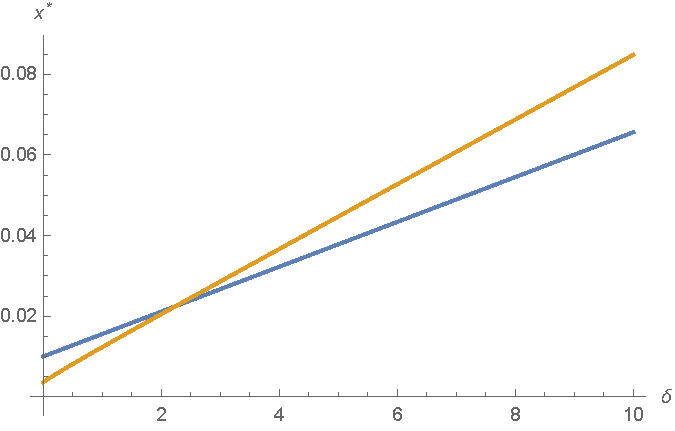
\includegraphics[width=0.45\textwidth]{Prob2_CapOpt/xopt_delta.pdf}}
		\subfigure[$\sigma \in (0,1)$]{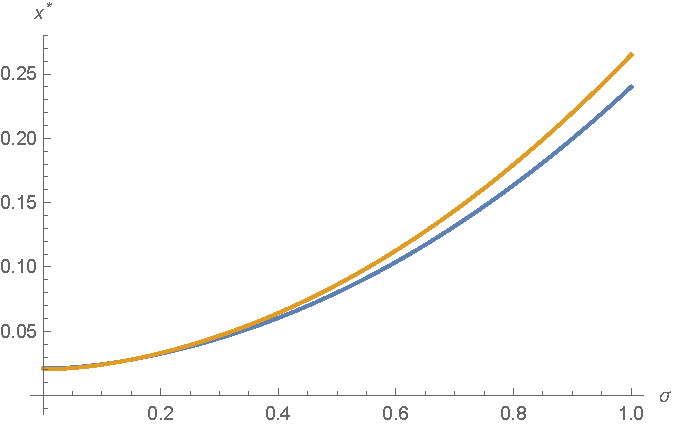
\includegraphics[width=0.45\textwidth]{Prob2_CapOpt/xopt_sigma.pdf}}
	\end{subfigmatrix}
	\caption{Threshold value with respect to the benchmark model (blue) and the capacity optimized model (orange) and parameters with which $x^*_B$ increases.}
	\label{fig:2_x2}
\end{figure}

On Figure \ref{fig:2_x2}, we obtained similar results to the ones on Section 2. Both threshold values increase with sensibility parameter $\delta$ and volatility $\sigma$. The first one is justified by the fact that a higher $\delta$ means a bigger investment, and thus it will only be made, if there's also a huge demand of the product. The second one is justified by the huge uncertainty of the demand. Since it has a high variance, the demand has a great amplitude of values, which delays the investment decision, only made when the demand reaches a high level. This is in accordance to what is described in \cite{dixit:book}.


\begin{figure}[!htb]
	\begin{subfigmatrix}{2}
		\subfigure[$\mu \in ( -r,r )$ ]{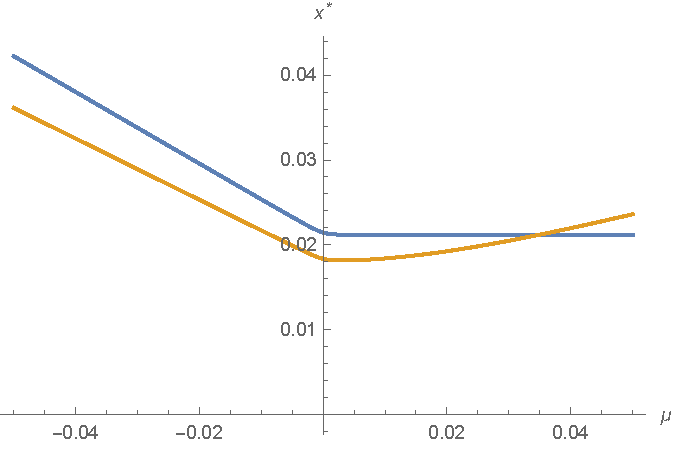
\includegraphics[width=0.45\textwidth]{Prob2_CapOpt/xopt_mu.pdf}}
		\subfigure[$\theta \in (1,10)$]{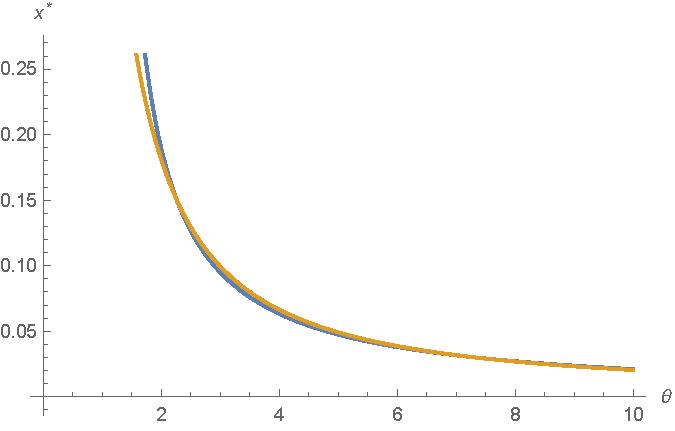
\includegraphics[width=0.45\textwidth]{Prob2_CapOpt/xopt_theta.pdf}}
	\end{subfigmatrix}
	\caption{Threshold value with respect to the benchmark model (blue) and the capacity optimized model (orange) and parameter with which  $x^*_B$ decreases.}
	\label{fig:2_x3}
\end{figure}

On Figure \ref{fig:2_x3} we see that, similarly to what happened on Section 2, both threshold levels decrease with innovation level. Although the threshold level associated to the Benchmark Model decreases with $\mu$ in what seems to be a linear way for negative values of $\mu$ and almost negligible for positive values of $\mu$, the same doesn't happen to the threshold level associated to the capacity optimization model. This last one, seems to increase for positive values of $\mu$. 

%The same happened considering other values for parameters $K_0, \ \alpha, \ \delta, \ \theta$. Regarding $\sigma$, we obtained that when increasing the volatility, the value of $\mu$ associated with the stationary point happens for values of $\mu$ greater than 0.

\begin{figure}[!htb]
	\begin{subfigmatrix}{3}
		\subfigure[$r \in (\mu,1)$, $\mu=0.01$ and $\sigma=0.9$]{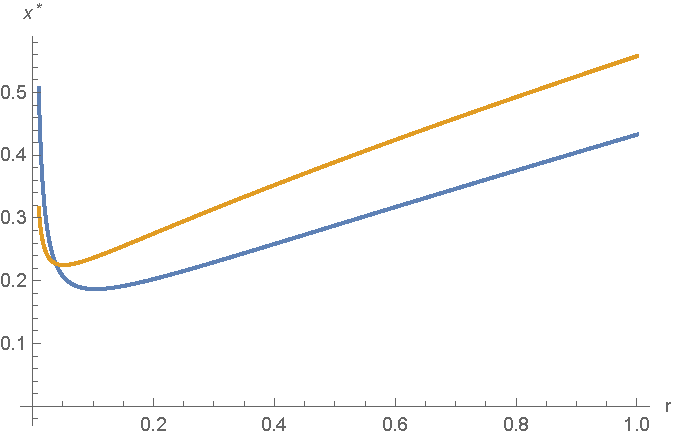
\includegraphics[width=0.32\textwidth]{Prob2_CapOpt/xopt_r.pdf}}
		\subfigure[$K_0 \in ( 0, \frac{1}{\alpha}=100 )$ ]{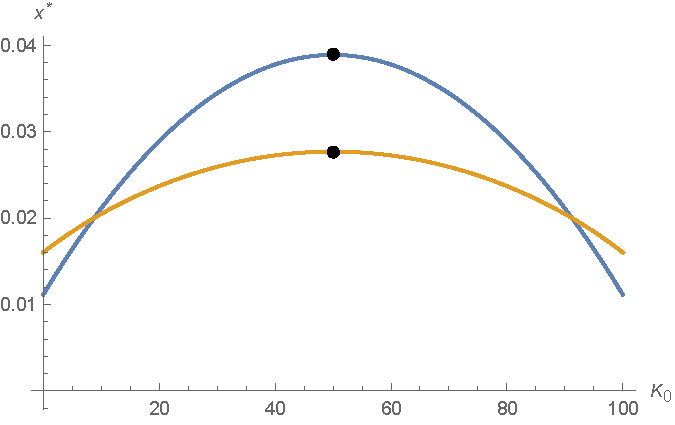
\includegraphics[width=0.32\textwidth]{Prob2_CapOpt/xopt_k0.pdf}}
		\subfigure[$K_1 \in (0, \frac{\theta}{\alpha}=1000 )$]{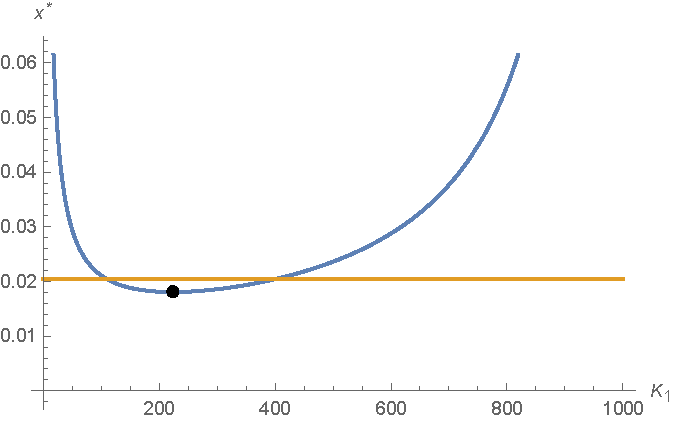
\includegraphics[width=0.32\textwidth]{Prob2_CapOpt/xopt_k1.pdf}}
	\end{subfigmatrix}
	\caption{Threshold value with respect to the benchmark model (blue) and the capacity optimized model (orange) and parameters with which  $x^*_B$ has a non-monotonic behaviour.}
	\label{fig:2_x1}
\end{figure}

On Figure \ref{fig:2_x1} we have that a non-monotonic behaviour was also observed on parameters $r$, $K_0$ and $K_1$, being this last one only valid for the Benchmark Model.
%On Figure \ref{fig:2_x1}, we observe that both threshold level behave in a non-monotonic way with $r$ and $K_0$.

On the leftmost plot we can see that a minimum demand threshold is observed for small values of discount rate $r$. Unfortunately we couldn't derive its analytical expression.

Interestingly, as seen on the plot located at the center, regarding the capacity of \textit{old} product, a maximum demand threshold is observed for both models when the capacity level $K_0$ is exactly equal to $\frac{1}{2 \alpha}$. This values comes from the expression $\alpha K_0 \pi_0=\alpha K_0 (1-\alpha K_0)$ included on both expressions of $x_B^*$ \eqref{2_xB} and $x^*_C$ \eqref{eq:prob2_xC}.

Regarding parameter $K_1$, its value doesn't affect threshold $x^*_C$, since it takes into account the optimal capacity $K^*_C$. However, when it comes to the threshold $x^*_B$ we have that it achieves a minimum value at $K_1=\frac{\pi_0+\sqrt{\alpha \pi_0(\pi_0+\delta \theta r)}}{r\alpha \delta}$, as it's represented on the bottom plot. Note that the standard value considered was $K_1=100$ and that it's associated a threshold $x_B^*$ smaller than the threshold $x_C^*$. This is one of the reasons why the demand threshold $x_B^*$ appears to be smaller than $x_C^*$ in most cases. However as showed in Figure \ref{fig:Kvar} (b), we have that the value function $F^*$ (associated to the threshold $x_C^*$) will always be greater than the value function $F$ (associated to the threshold $x_B^*$).
	
	\begin{figure}[!htb]
		\begin{subfigmatrix}{2}
			\subfigure[$\alpha \in (0,1)$ and $\theta=10>\frac{K_1}{ K_0^2} (K_0+K_1 r \delta)$]{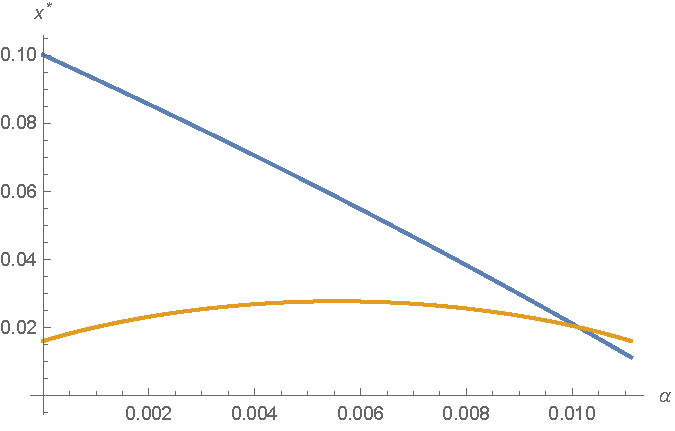
\includegraphics[width=0.45\textwidth]{Prob2_CapOpt/xopt_alpha_O.pdf}}
			\subfigure[$\alpha \in (0,1) $ and $\theta=1<\frac{K_1}{ K_0^2} (K_0+K_1 r \delta)$]{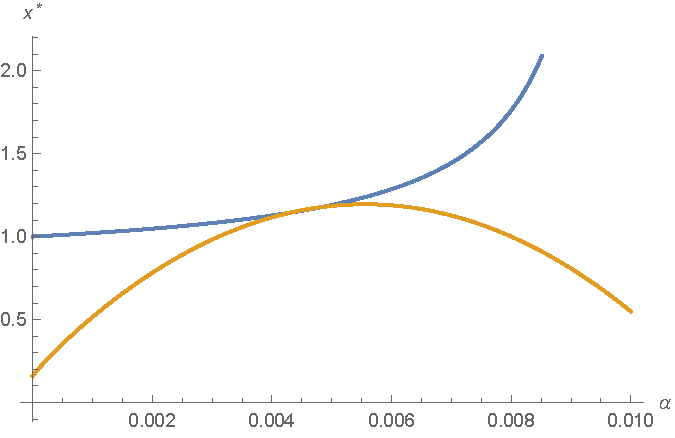
\includegraphics[width=0.45\textwidth]{Prob2_CapOpt/xopt_alpha_op.pdf}}
		\end{subfigmatrix}
		\caption{Threshold value with respect to the benchmark model (blue) and the capacity optimized model (orange) and sensibility parameter $\alpha$.}
		\label{fig:2_x4}
	\end{figure}
	
	On Figure \ref{fig:2_x4} it's represented the behaviour of $x^*_B$ with $\alpha$, as written on Proposition \label{3_prop2}. Considering the fixed values considered before, we obtain a $\theta$-threshold equal to $\frac{K_1}{ K_0^2} (K_0+K_1 r \delta)=1.23457$. One can see on Figure \ref{fig:2_x4} when that testing for innovation levels greater (leftmost) and smaller (rightmost) than the mentioned threshold, we verify what was deduced: that $x^*_B$ behaves in either an increasing or decreasing way with $\alpha$ for certain levels of innovation, while $x_C^*$ always behave in a non-monotonic way.
	%Note that on most of the plots you have that the threshold $x_C^*$ has an associated capacity level ($K^*(x_C^*)$) greater than the one considered ($K_1=100$), resulting in values $x^*_B$ smaller than $x_C^*$, contrarily to what happened on the previous section.

\subsection{Optimal Capacity Level}

Now we analyse optimal capacity level $K^*_C$, that is given by evaluating $K^*$ on demand level $x^*_C$ and as it is written in \eqref{3_K*}.

\begin{prop}
Optimal capacity level $K^*_C$ increases linearly asymptotically with $\theta$ and does not have a monotonic behaviour with $K_0$. 
\end{prop}

\textbf{Proof:}

Regarding innovation level $\theta$, assuming that it has no upper limit, it's possible to evaluate its behaviour asymptotically. Denoting $\theta_K:=\frac{\sigma ^2 \left(\sqrt{\delta ^2 r^2}+\delta  r\right)}{\alpha  \left(2 \sigma ^2 \sqrt{\delta ^2 r^2}+\delta  r \left(\sigma ^2 (\phi +1)-2 \mu \right)\right)}>0$, we obtain that $K^*_C$ increases on order of $\theta_K \theta$, that is,
$$K^*_C(\theta) \sim \theta_K \theta \ \Leftrightarrow \ \lim_{\theta \to \infty}  \frac{K^*_C}{\theta_K \theta}=1 $$


The non monotonic behaviour of $K^*_C$ with $K_0$ will be showed hereunder in the obtained plots.
\begin{flushright}
	$\square$
\end{flushright}

Although it wasn't possible to derive any (strong) analytical solution about te behaviour of the other parameters, numerically we obtain robust results. By manipulating each parameter, using command \texttt{Manipulate}, we obtained no different behaviours from the ones showed hereunder.

The results obtained regarding parameters $\mu, \ \sigma,\ r, \ \alpha$ and $\theta$  were similar to the ones obtain for the optimal capacity level on the previous section.  Since $K^*_C$ depends on value $x_C^*$, it is expected to observe similiar behaviours regarding the studied parameters. 


\begin{figure}[!htb]
	\centering
	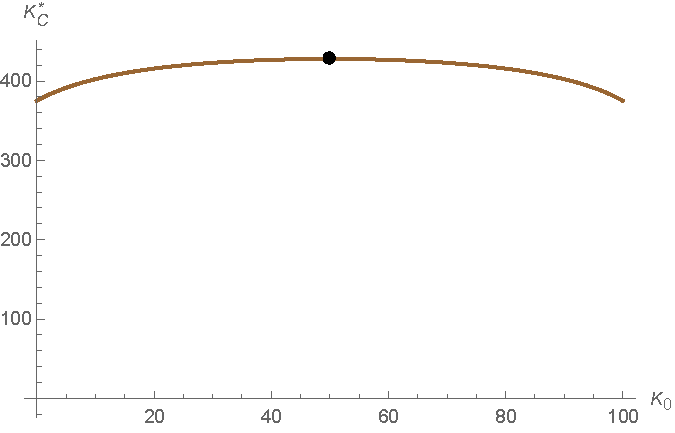
\includegraphics[width=0.45\textwidth]{Prob2_CapOpt/koptx_k0.pdf}
	\caption{Optimal capacity regarding the threshold value $x^*_C$ considering capacity levels $K_0 \in [0, 100)$ and its highest values at $\frac{1}{2 \alpha}=50$ (black).}
	\label{fig:2_k0}
\end{figure}

Starting with the capacity level of the \textit{old} product $K_0$, on Figure \ref{fig:2_k0}, we obtained that the highest optimal capacity level $K^*_C$ happens for $K_0=\frac{1}{2 \alpha}$. This is motivated by the results obtained for $x^*_C$, as seen on Figure \ref{fig:2_x1}, which also reaches its highest value at $\frac{1}{2 \alpha}$.


\begin{figure}[!htb]
	\begin{subfigmatrix}{3}
		\subfigure[$\mu \in ( -r,r )$ ]{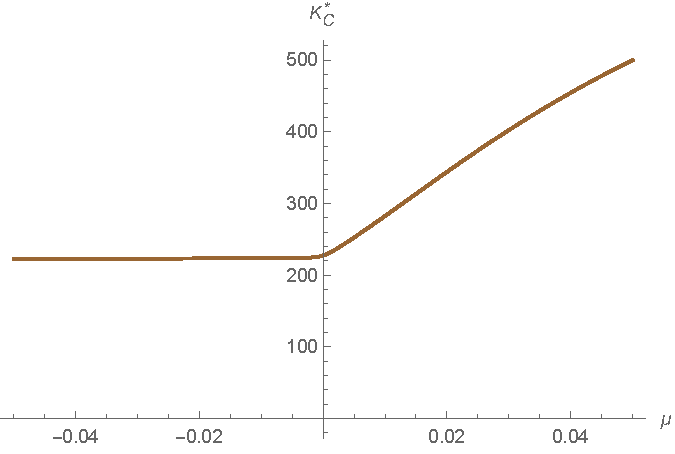
\includegraphics[width=0.32\textwidth]{Prob2_CapOpt/koptx_mu.pdf}}
		\subfigure[$\sigma \in (0,1)$]{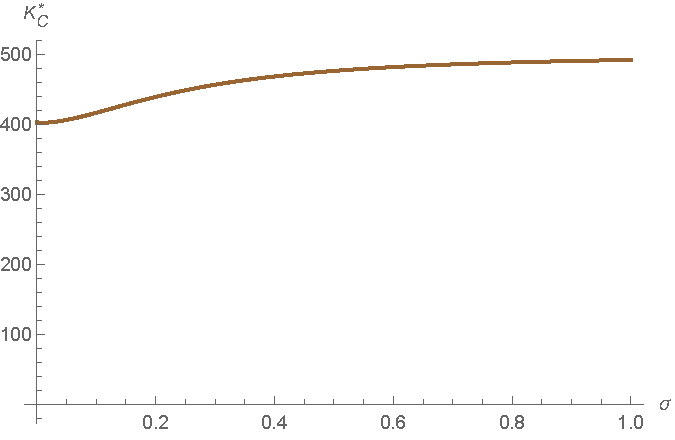
\includegraphics[width=0.32\textwidth]{Prob2_CapOpt/koptx_sigma.pdf}}
		\subfigure[$ \theta \in ( 1, 10 )$]{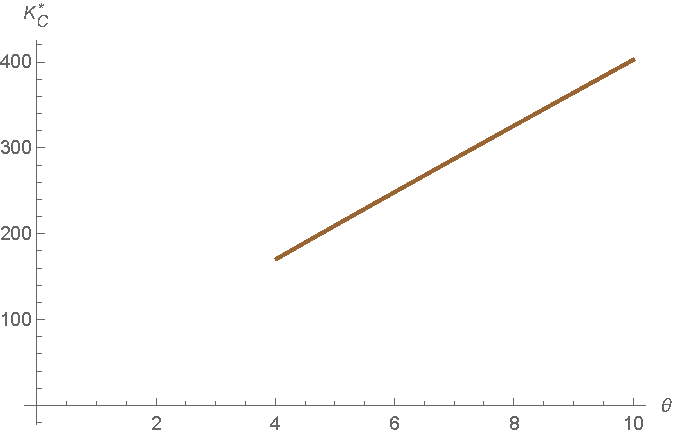
\includegraphics[width=0.32\textwidth]{Prob2_CapOpt/koptx_theta.pdf}}
	\end{subfigmatrix}
	\caption{Optimal capacity regarding the threshold value $x^*_C$ and increasing parameters $\mu, \ \sigma$ and $\theta$}
	\label{fig:2_k1}
\end{figure}

On Figure \ref{fig:2_k1}, we obtain that $K^*_C$ increases with both drift, volatility and innovation level, as it happened in the previous section. Note that again that, contrary to what happens for positive drift values, the growth of $K^*_C$ with $\mu$ is barely noticeable for negative values of $\mu$. This is related to the inverse relationship between $K^*_C$ and $x_C^*$.


Also note that $K^*_C$ seems to increase linearly with $\theta$, being in accordance to the asymptotical behaviour of $K_C^*$ with $\theta$ previously deduced.

\begin{figure}[!htb]
	\begin{subfigmatrix}{3}
		\subfigure[$ \delta \in (0,10)$]{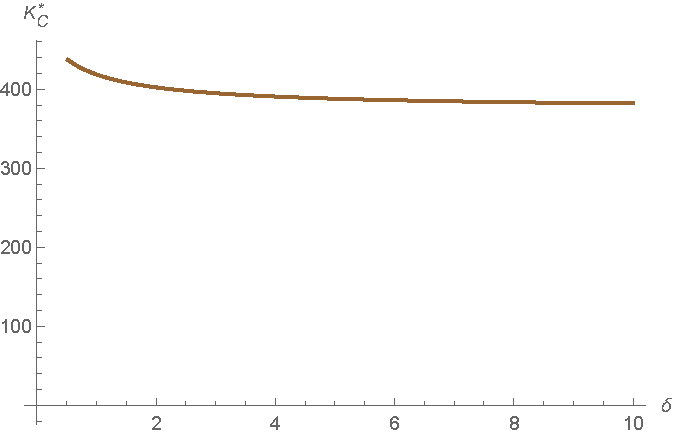
\includegraphics[width=0.32\textwidth]{Prob2_CapOpt/koptx_delta.pdf}}
		\subfigure[$ r \in ( \mu, 1 )$]{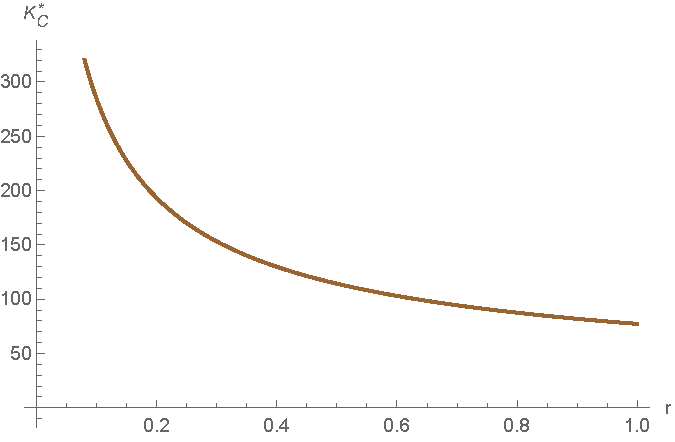
\includegraphics[width=0.32\textwidth]{Prob2_CapOpt/koptx_r.pdf}}
		\subfigure[$ \alpha \in (0,1)$]{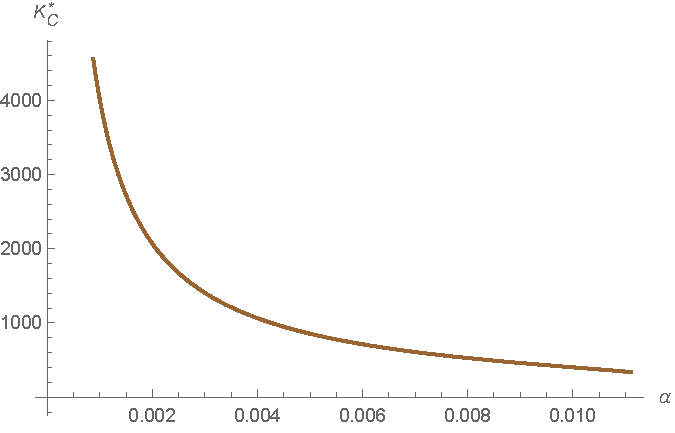
\includegraphics[width=0.32\textwidth]{Prob2_CapOpt/koptx_alpha.pdf}}
	\end{subfigmatrix}
	\caption{Optimal capacity regarding the threshold value $x^*_C$ and decreasing parameters $\delta, \ r$ and $\alpha$.}
	\label{fig:2_k3}
\end{figure}

Regarding  sensibility parameter $\delta$, discount rate $r$ and sensibility parameter $\alpha$, we have on Figure \ref{fig:2_k3} that $K^*_C$ decreases with them, as happened in the previous section.



